%source mathadata
Luc hésite entre remplir sa gourde à la fontaine A ou à la fontaine B. On cherche à déterminer quelle fontaine est la plus proche de Luc.

	\begin{MADenumerate}
		\begin{multicols}{2}

			\item Vérifier que les coordonnées de Luc sont $L(4\,;\,5)$ puis placer la fontaine A en $A(1\,;\,3)$ et la fontaine B en $B(5\,;\,1)$.
			\item \begin{enumerate}

				\item Ajouter le point $H(1\,;\,5)$.
				\item Les axes des abscisses et des ordonnées sont perpendiculaires. Que peut-on en déduire pour le triangle $AHL$ ?
				\item En lisant les distances $AH$ et $HL$, calculer la distance $AL$.
			\end{enumerate}
			\item Calculer de même la distance $BL$ pour la fontaine B en ajoutant un point $K$ bien choisi (demander un point au professeur au bout de 5 minutes si on ne trouve pas).
			\item Comparer les distances $AL$ et $BL$. Quelle fontaine doit choisir Luc ?

			\columnbreak

			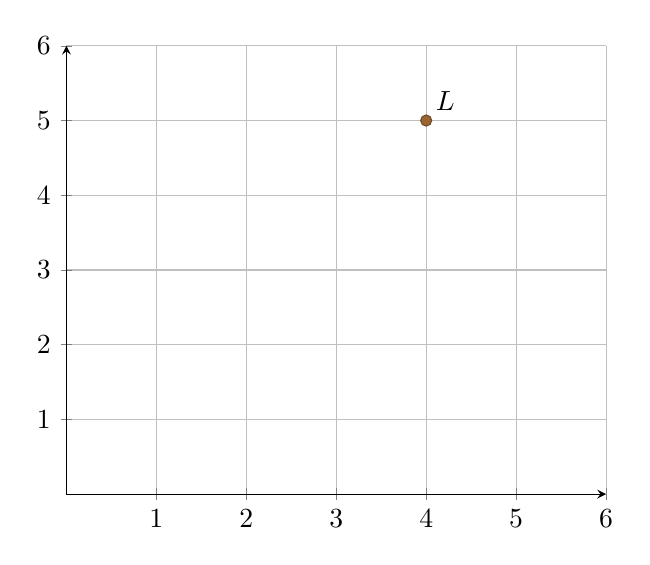
\begin{tikzpicture}
				\begin{axis}[
						xmin=0, xmax=6, ymin=0, ymax=6,
						grid=major,
						axis lines=middle,
						xtick distance=1, ytick distance=1,
						clip=false % utile si tu ajoutes un pin/label qui sort du cadre
					]
					% un seul point en (2,6)
					\addplot+[only marks, mark=*, mark size=2pt,opacity=0] coordinates {(1,4)};
					% optionnel : une étiquette
					\node[anchor=south west,opacity=0] at (axis cs:1,4) {$A$};
					\addplot+[only marks, mark=*, mark size=2pt,opacity=0] coordinates {(5,2)};
					\node[anchor=south west,opacity=0] at (axis cs:5,2) {$B$};

					\addplot+[only marks, mark=*, mark size=2pt,opacity=1] coordinates {(4,5)};
					\node[anchor=south west] at (axis cs:4,5) {$L$};
				\end{axis}
			\end{tikzpicture}

		\end{multicols}

	\end{MADenumerate}
